\documentclass[12pt,a4paper,oneside]{ctexart}
\input{结构设定.tex}
\title{\textbf{社区识别\\基于无桩共享单车“潮汐”特征的时空聚类}}

%自定义一个keywords
\newcommand{\keywords}[1]{\par\noindent\textbf{关键词:} #1}
\author{张浩怡、潘凌志}

\date{\today}

\begin{document}

\maketitle
\begin{abstract}
\textit{上海市的共享单车企业主要采用无桩共享单车的运营模式,这在为市民生活提供便利的同时,也因单车在地区间的流入流出具有较大的随机性和不确定性,导致了显著的“潮汐”现象。这种现象对市民的日常生活及城市交通管理带来了负面影响。因此,针对市民停车点的聚类划分,实施区域化的管理与调度显得尤为重要。}

\textit{本文实现了一种基于时空约束的网络图聚类算法,该算法结合了空间因素(如地理位置和地理环境特征)与时间因素(如历史订单数据),通过设置一定的距离阈值即可实现电子围栏的多尺度聚类划分。以深圳市的停车点为实验对象,在500米距离阈值条件下进行聚类分析,结果表明,该算法能够有效地将具有相似时空特征的停车点归类到同一社区簇中,并使得单车流动主要集中在划分后的社区内部。}

\textit{在完成社区划分的基础上,本文进一步挖掘了单车的潮汐特征,成功识别并定位了单车使用的热点区域,提供了城市发展的新视角。研究结果为停车点规划和共享单车的区域化管理与调度提供了科学依据,同时也为单车企业在不同地区的个性化商业运营提供了参考。}
\end{abstract}

\keywords{无桩共享单车,数据挖掘,时空约束,多尺度聚类,使用模式,社区识别}

\section{项目背景及意义}
\subsection{项目背景}

共享单车的兴起,使得“共享单车+地铁”“共享单车+公交”已成为城市通勤的主要接驳方式。但共享单车的“潮汐效应”也成为共享单车管理和资源调配的“痛点”和“难点”\cite{ChatGPT2024}。具体而言,自行车的“借还”存在特定时间段的波峰波谷现象,在城市下班的早晚高峰“借不到,停不好”,由此造成了市民生活的不便利以及公共资源的浪费。因此,如何发现并理解共享单车的“潮汐”规律,对于共享单车的有序规范发展,优化用车体验和环境等具有重要意义。

\subsection{相关工作}

相对于有桩“公共自行车”,无桩共享单车的出现较晚\cite{高楹2018北京市摩拜}。目前相关研究大多关注有桩“公共自行车”的资源分配问题。这得益于有桩共享单车较长的历史背景、固定停车桩位带来的问题化简以及长期研究的积累。具体而言,这些研究可分为两类,一类注重于公共自行车用车量的影响因素。不同学者采用不同的方法进行共享单车聚类问题的研究。如El-Assi等(2017)基于经验探讨了有桩共享单车系统的使用模式,包括早晚高峰期间的租还车行为\cite{el2017}。随着数据收集技术的发展,研究开始利用大数据分析来识别热点区域。(高楹等,2018)\cite{高楹2018北京市摩拜}。

\subsection{项目意义}

综上所述,已有研究主要关注有桩共享单车的用车影响因素以及站点之间的调度方法。而由于无桩共享单车不存在集中的站点,车辆的起止位置仅与用户个人的出行目的有关,分散于城市中,导致其形成的网络极其复杂;而其流动性更强的特点也导致存车数量难以实时监控。因此,我们希望可以系统研究无桩共享单车的时空分布特征及影响因素,并提出针对性、可行性高的优化策略。

\section{问题描述}

\subsection{问题简述}

基于以上内容,我们提炼出本文关注的问题,如下所示:
\begin{enumerate}
    \item 问题一:在微观尺度上,识别并聚类具有不同“潮汐”特征的源汇区域。结合土地利用分类数据,判断各个土地类型对共享单车使用情况的影响。
    \item 问题二:在宏观尺度上,进行网格间的单元调度。基于网格化数据和土地利用类型数据,思考局部共享单车资源调度方法。
\end{enumerate}

\subsection{问题分析}
具体而言,问题一属于时空聚类研究,系数据挖掘问题,而问题二属于资源调度研究,则需要采用运筹规划的算法来解决。考虑到课程主题以及作者的时间精力,本文将以问题一作为主要的目标,而问题二则作为在实现问题一的基础上再做拓展。
\subsection{技术路线}
\begin{figure}[H]
    \centering
    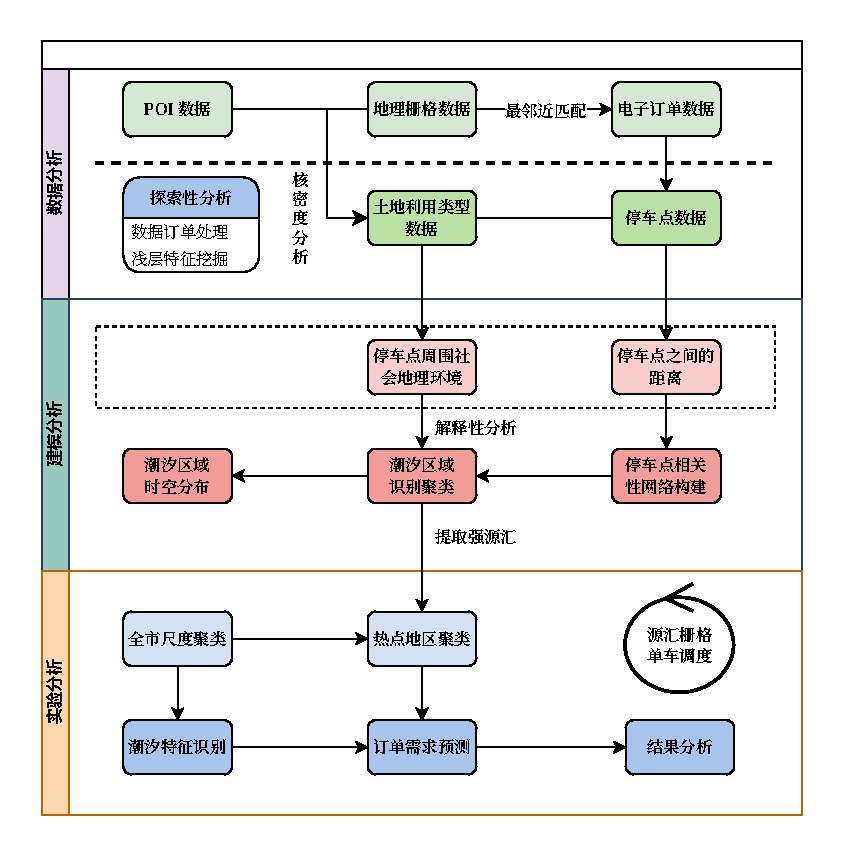
\includegraphics[width=\linewidth]{Figs/技术路线.pdf}
    \caption{技术路线}
    \label{fig:技术路线}
\end{figure}
\section{数据集}

\subsection{数据集来源}

本文使用到的数据主要来自两部分,
\begin{enumerate}
    \item 2021深圳开放数据应用创新大赛”的数据。来源于深圳市政府数据开放平台(下称平台,相关链接: \href{https://opendata.sz.gov.cn/data/api/toApiDetails/29200_00403627}{https://opendata.sz.gov.cn})。数据包含 2021 年 1 月 至 8 月 的部分共享单车订单数据,共 8 个数据项,数据类型均为字符串型,全量为 条,为确保用户隐私安全,数据已进行必要的脱敏处理。经纬度基于 bd09 坐标系。
    \item 深圳市土地使用情况兴趣点(POI,Point of Interact)。来源于公开网络平台 POI 数据(相关链接:\href{https://www.poi86.com/poi/amap/city/440300.html}{https://www.poi86.com})。数据包含 2021 年深圳市各区的土地使用情况。共 23 种使用用途,全量 3068185 条。

\end{enumerate}

\subsection{数据集构成}

数据集构成如下表所示,
\begin{table}[H]

\centering

\caption{实验数据清单}
\vspace{12pt}
\label{tab:experimental_data_list}
\begin{tabular}{@{}ccccc@{}}
\toprule
数据名称                           & 数据时间                                                                 & 数据规模                         & 字段名称          & 字段含义     \\ \midrule
\multirow{9}{*}{深圳市共享单车订单数据}   & \multirow{9}{*}{\begin{tabular}[c]{@{}c@{}}2021年\\ 1月1日-8月 31日\\ 0:00 - 24:00\end{tabular}} & \multirow{9}{*}{244,638,540 条}                     & START\_TIME   & 开始时间     \\
                               &                                                                                          &                                                  & END\_TIME     & 结束时间     \\
                               &                                                                                          &                                                  & START\_LAT    & 开始纬度/°    \\
                               &                                                                                          &                                                  & START\_LNG    & 开始经度/°   \\
                               &                                                                                          &                                                  & END\_LAT      & 结束纬度/°   \\
                               &                                                                                          &                                                  & END\_LNG      & 结束经度/°   \\
                               &                                                                                          &                                                  & USER\_ID      & 用户 ID    \\
                               &                                                                                          &                                                  & COM\_ID       & 企业 ID    \\ \cmidrule(l){1-5}
\multirow{3}{*}{深圳市 POI 数据} & \multicolumn{1}{l}{\multirow{3}{*}{2021年8月}}                                             & \multicolumn{1}{l}{\multirow{3}{*}{3,068,185 条}} & POI\_TYPE     & 地物类别  \\
                               & \multicolumn{1}{l}{}                                                                     & \multicolumn{1}{l}{}                             & LATITUDE      & 纬度/°     \\
                               & \multicolumn{1}{l}{}                                                                     & \multicolumn{1}{l}{}                             & LONGITUDE     & 经度/°     \\ \bottomrule
\end{tabular}
\end{table}

\subsection{符号说明}

本文使用到的数学记号如下表所示:

\begin{table}[H]
\centering
\begin{tabular}{cc}
\toprule
\textbf{符号} & \textbf{解释} \\
\midrule
$t_0^{(i)}$ & 第i条数据开始时间 \\
$t_1^{(i)}$ & 第i条数据结束时间 \\
$\phi_0^{(i)}$ & 第i条数据开始纬度(度) \\
$\lambda_0^{(i)}$ & 第i条数据开始经度(度) \\
$\phi_1^{(i)}$ & 第i条数据结束纬度(度) \\
$\lambda_1^{(i)}$ & 第i条数据结束经度(度) \\
$p^{(i)}$ & 第i条数据地物类别 \\
$R$ & 地球半径\\
\bottomrule
\end{tabular}
\caption{数据字段说明}
\label{tab:data_fields}
\end{table}

\section{数据预处理与探索性分析}

% What do you do
% Why do this
% How do this
\subsection{数据抽样}

实验抽取了8月11日至8月18日,共10,178,948条数据作为实际用例数据。

一个理想的数据集应当具有时效性以及可操作性。一方面,原数据集总规模近 2.5 亿,存储到本地数据库约 24.5G,同时时间跨度超过半年,如此体量并不利于数据的分析和特征的挖掘;而过短的时间范围则不利于规律的发现。因此选取具有普遍意义的城市生活周期 —— 一周(吴兵,2003\cite{吴兵2003城市生命周期})作为时间的跨度兼顾实验需求。这同时回答了为什么不使用随机抽样。

另一方面,一年内,8月的市民活跃度处于一个较高的水平,该月的数据具有更强的代表性。同时,2021年7月至9月期间,台风多次登陆深圳,因此8月上旬下旬受风雨影响较大,自行车使用量有明显下降;而8月中旬则处于台风登陆的间歇期\cite{CMA_API_Documentation},为阴天或晴天,受台风影响较小。基于上述考虑,选取8月中旬(11日至18日)作为用例数据。

\subsection{数据清理}

检查后并没有发现缺失值,通过 \texttt{START\_TIME, END\_TIME, START\_LAT, START\_LNG, END\_LAT, END\_LNG},结合 POI 数据,构建得到三个特征:运行时间\texttt{running\_time}、运行位移\texttt{running\_dis}、运行速度\texttt{running\_speed}。将运行时间小于 1 分钟,超出 2 h 的数据点,运行位移小于 1 m或超出深圳市边界的数据点以及运行速度超过 25 km/h 的数据点删除。
计算公式如下:
\begin{align}
& running\_time = t_1 - t_0 \\
& \begin{cases}\label{Haversine}
    &a= \sin^2\left(\frac{\phi_1 - \phi_0}{2}\right) + 
    \cos(\phi_0) \cdot \cos(\phi_1) \cdot 
    \sin^2\left(\frac{\lambda_1 - \lambda_0}{2}\right) \\
&c = 2 \cdot \arctan2\left(\sqrt{a}, \sqrt{1-a}\right) \\
&running\_dis = R \cdot c
\end{cases}\\
& running\_speed = \dfrac{running\_dis}{running\_time}
\end{align}

就运行时间而言,现行的共享单车策略允许消费者在 1 分钟内无偿结束骑行,同时运行时间短于1分钟的数据对“潮汐”的影响微弱,因此可以删除。将确定下界的运行时间以分钟为单位取对数前后绘制分布图如下所示:
\begin{figure}[H]
    \centering
    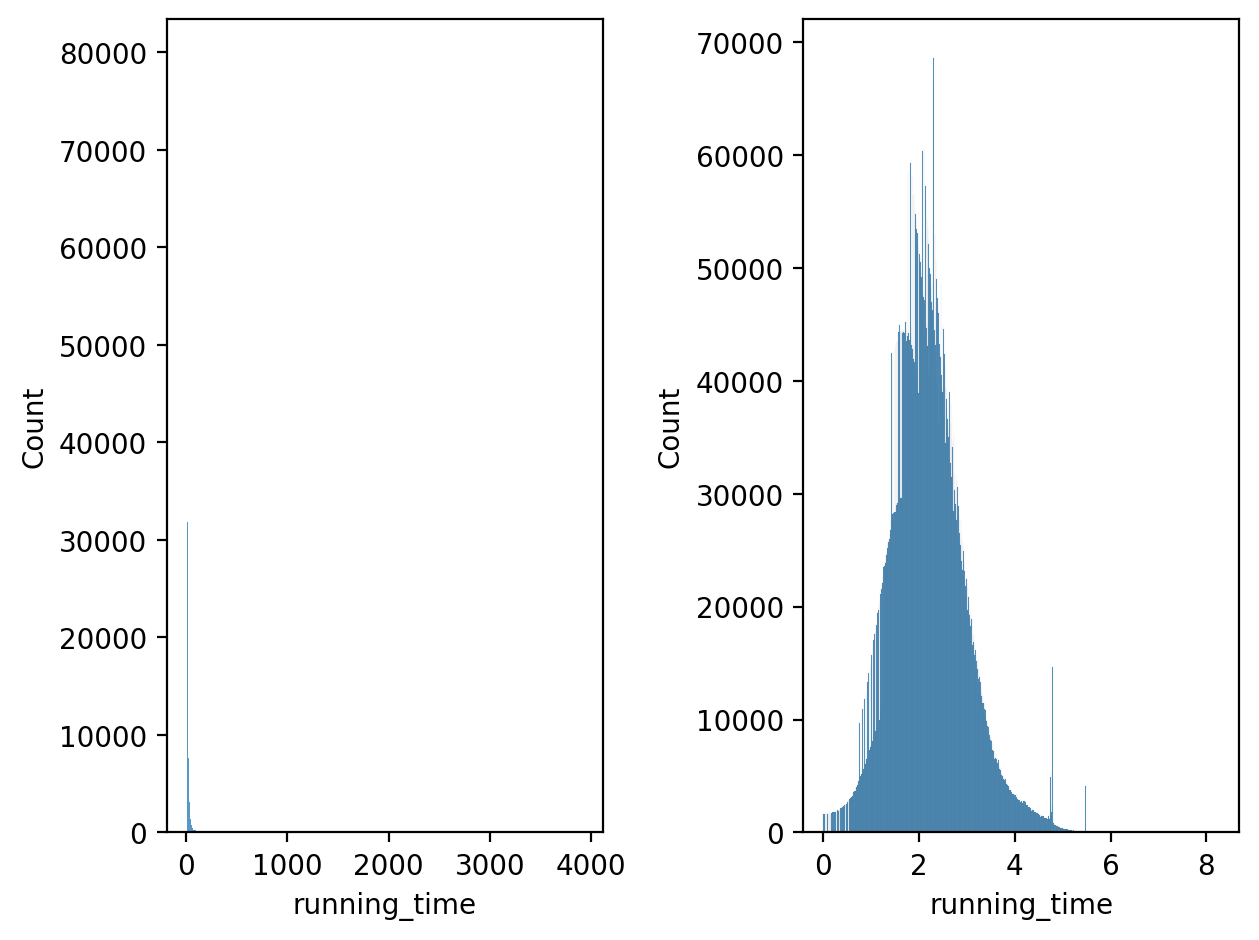
\includegraphics[width=0.8\textwidth]{Figs/运行时间分布图.png}
    \caption{运行时间分布(左:取对数前,右:取对数后)}
    \label{fig:运行时间分布}
\end{figure}


分布呈现倒锥型,数据呈现出一个明显的峰值,且右侧有较长的尾部,且存在一个明显的突起。经检验,近似服从正态分布,因此以 $\mu + 3\sigma$ 作为上界。这既符合了正态分布的 $3\sigma$ 原则,同时也保留了具有显著现实意义的突起,为后续分析提供更多元的视角支撑。处理后剩余 9,937,790 条数据。 

对于运行距离,理想的构建方法是通过街道分布等得到准确的一个准确的路程。但这样的计算复杂度过大,因此选取更容易计算,考虑了地球形状的 Haversine 公式(即公式(\ref{Haversine}))计算两点间的距离。具体的实现我们借助了\texttt{Haversine}中的函数,并借助 \texttt{NumPy} 的矢量化操作。

之后仿照运行时间的过程处理,将位移小于 1m 的删除,取对数后发现符合正态分布,删去 $\mu + 3\sigma$ 之上的数据。结果展示如下:

\begin{figure}[H]
    \centering
    \subfloat[运行距离箱线图]{
        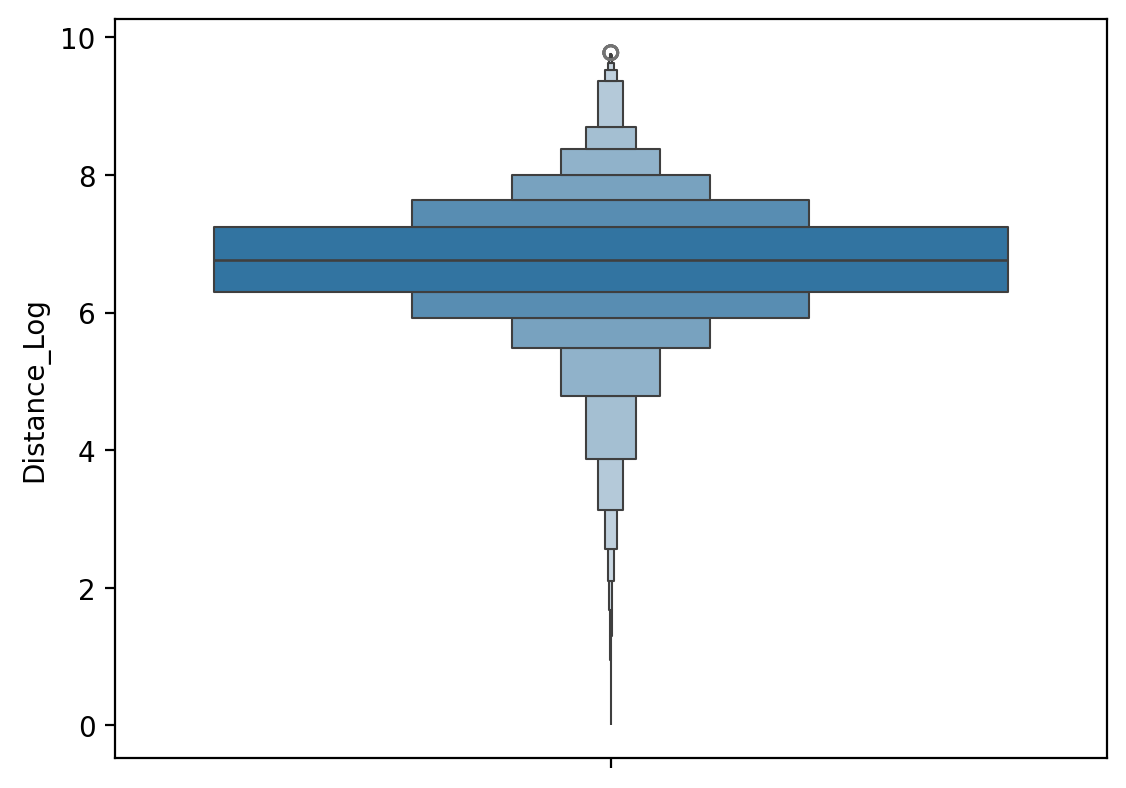
\includegraphics[width=0.48\textwidth]{Figs/dis.png}
        \label{fig:运行距离箱线图}
    }
    \subfloat[运行距离与运行时间双对数分布图]{
        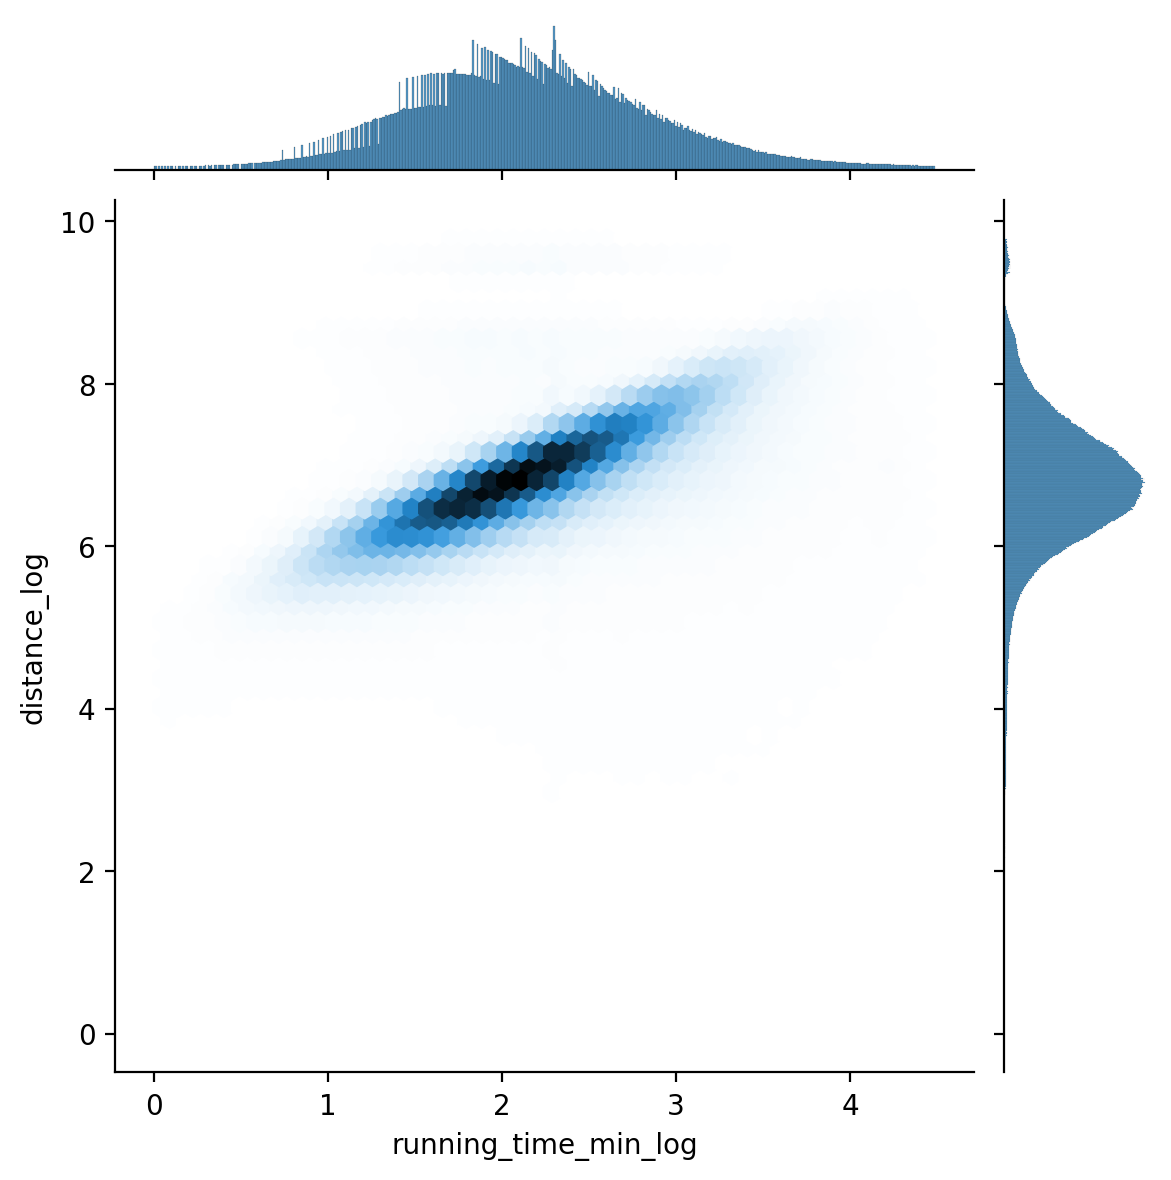
\includegraphics[width=0.48\textwidth]{Figs/时空因素.png}
        \label{fig:运行距离与运行时间双对数分布图}
    }
    \label{fig:combine}
\end{figure}


此外,在预实验中,我们发现一些位移点超出了深圳市边界,严重者偏移到了北京、中东等地,将此类数据删除。以 POI 数据构建了深圳的边界范围,并保留了一定的偏移值作为缓冲后边界如下所示:

\begin{figure}[H]
    \centering
    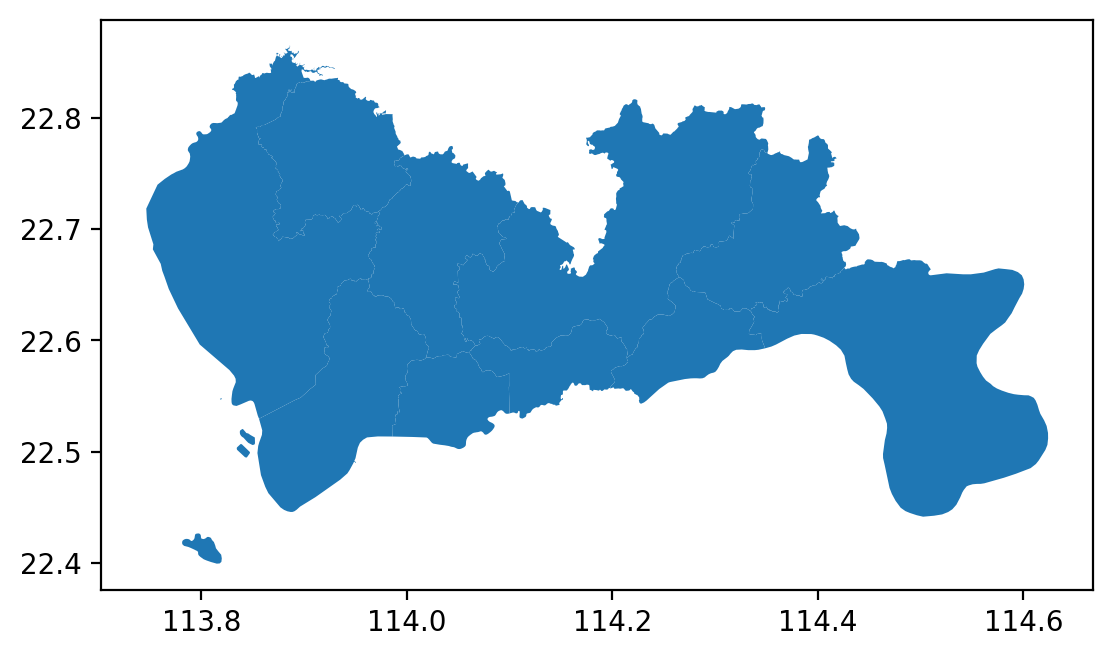
\includegraphics[width=\linewidth]{Figs/深圳市边界.png}
    \caption{深圳市边界}
    \label{fig:boundary}
\end{figure}

2019年4月,新的电动自行车强制性国家标准《电动自行车安全技术规范》\cite{GB17761-2018}开始施行,规定了电动自行车必须满足以下条件:最高设计车速不超过 25km/h。该规则对于公司设定共享单车的速度具有参考性质。事实上,经过我们的实验,共享单车的速度几乎不会超过 25km/h。

经过上述处理后,删去 544,602 条数据,剩余 9,634,346 条数据,变化率为 5.35\%。

\subsection{数据变换}

我们以 15 分钟为尺度,将一天内的时间划分为 96 个区间,对 \texttt{START\_TIME, END\_TIME} 进行等深离散化;对于地理信息则不做处理。

对\texttt{START\_TIME, END\_TIME} 做离散化处理主要是为了简化模型结构,减少计算复杂度。选择 15 分钟作为一个时间单位主要考虑到日常活动中的常见周期性模式,如交通流量、用户行为等\cite{吴兵2003城市生命周期}。同时,潮汐的峰值持续时间并不长,约 30 分钟(邝嘉恒,2022\cite{邝嘉恒2022吸引区域优化})。

需要注意的是,我们并没有使用 \texttt{One-Hot} 编码的形式存储。一方面,96 个时间区间以 \texttt{One-Hot} 编码存储后 \texttt{DataFrame} 的可读性很差;另一方面,该数据集并不是我们最终的实验数据集,\texttt{One-Hot} 对最终实验数据集的构建并不便捷,我们使用 \texttt{Slot} 作为新的属性。

对\texttt{START\_LAT, START\_LNG, END\_LAT, END\_LNG}不做处理主要是考虑到深圳特殊的地理性质。深圳位于东经 113°43′至 114°38′,北纬 22°24′ 至 22°52′ 之间。这意味着深圳的经度跨度大约为0.95度(约105公里),而纬度跨度约为0.467度(约52公里)。整体呈长方型。由于经纬度的地理长度并不一致,如果对经纬度进行归一化处理(如 Z-Score),则可能发生变形,丢失相当的地理信息。

以上的讨论是建立在原有的共享单车数据集上的,但“潮汐”现象是宏观上共享单车的集群表现。由于数据集的限制,我们无法得到每个共享单车的独特的运行特征,因此,有必要转化视角,将数据视角从共享单车转化到地理栅格上去,从地理栅格上发现、总结和利用“潮汐”现象。这是更为广义的数据规约。

\subsection{数据规约}

对由 POI 数据生成的深圳市边界\ref{fig:boundary} 使用 \texttt{TransBigData} 函数库以 100m 为作为空间分辨率,创建覆盖整个深圳市边界的地理栅格。使用\texttt{tbd.area\_to\_params}函数获取栅格化参数,然后利用\texttt{tbd.GPS\_to\_grids}方法将 GPS 点映射到对应的栅格上。

\begin{figure}
    \centering
    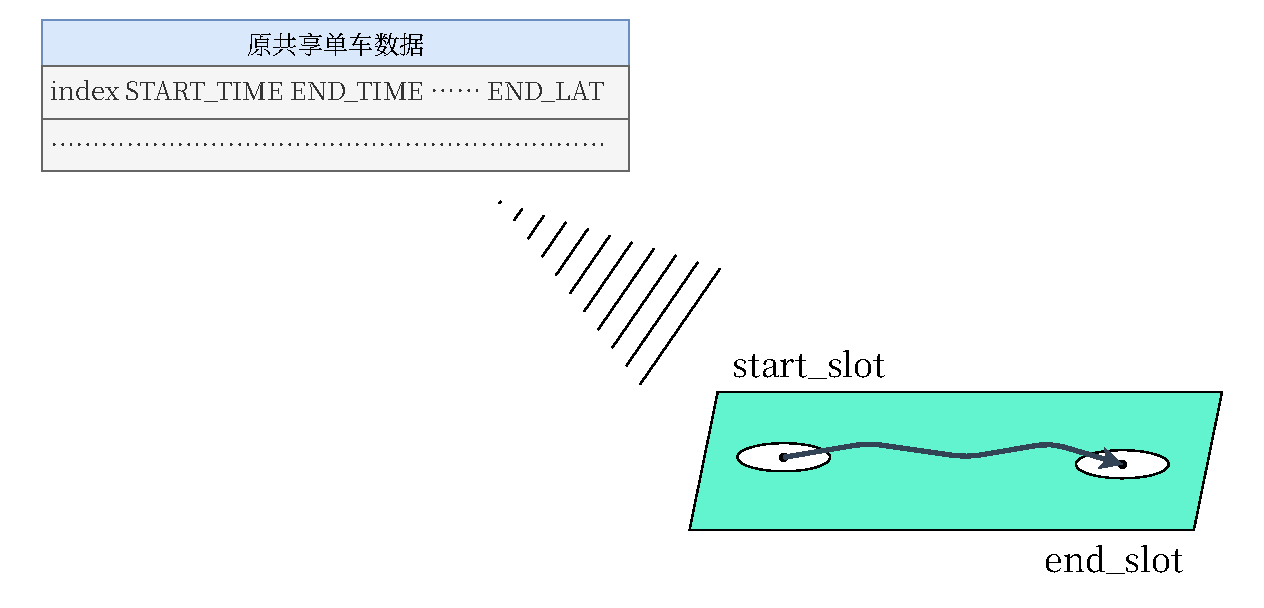
\includegraphics[width=\linewidth]{Figs/转化.pdf}
    \caption{广义数据规约示意图}
    \label{fig:trans}
\end{figure}

最终得到栅格:
\begin{equation}
    spacetime_{s}^{t} = \left[t_+^{(1)},t_-^{(1)},t_+^{(2)},t_-^{(2)} \cdots,t_+^{(i)}, t_-^{(-)} ,\cdots,t_+^{(96)},t_{-}^{(96)}\right]
\end{equation}

式中:s 代表当前栅格中心的地理位置,如 23 代表编号为 23 的地理栅格;t 代表当前栅格数据所属时间,如 4 代表该数据系第4天的数据;, $t_+^{(i)}, t_-^{(-)}$ 则代表处于 $t$ 区间时该地理栅格的共享单车的流量情况,其中 $+$ 代表流入,$-$ 代表流出,如 $t_{-}^{(8)}$ 代表该地理栅格在第 40 个区间(对应为 10:00 - 10:15时间段)内流出的共享单车数量。


\begin{figure}[H]
    \centering
    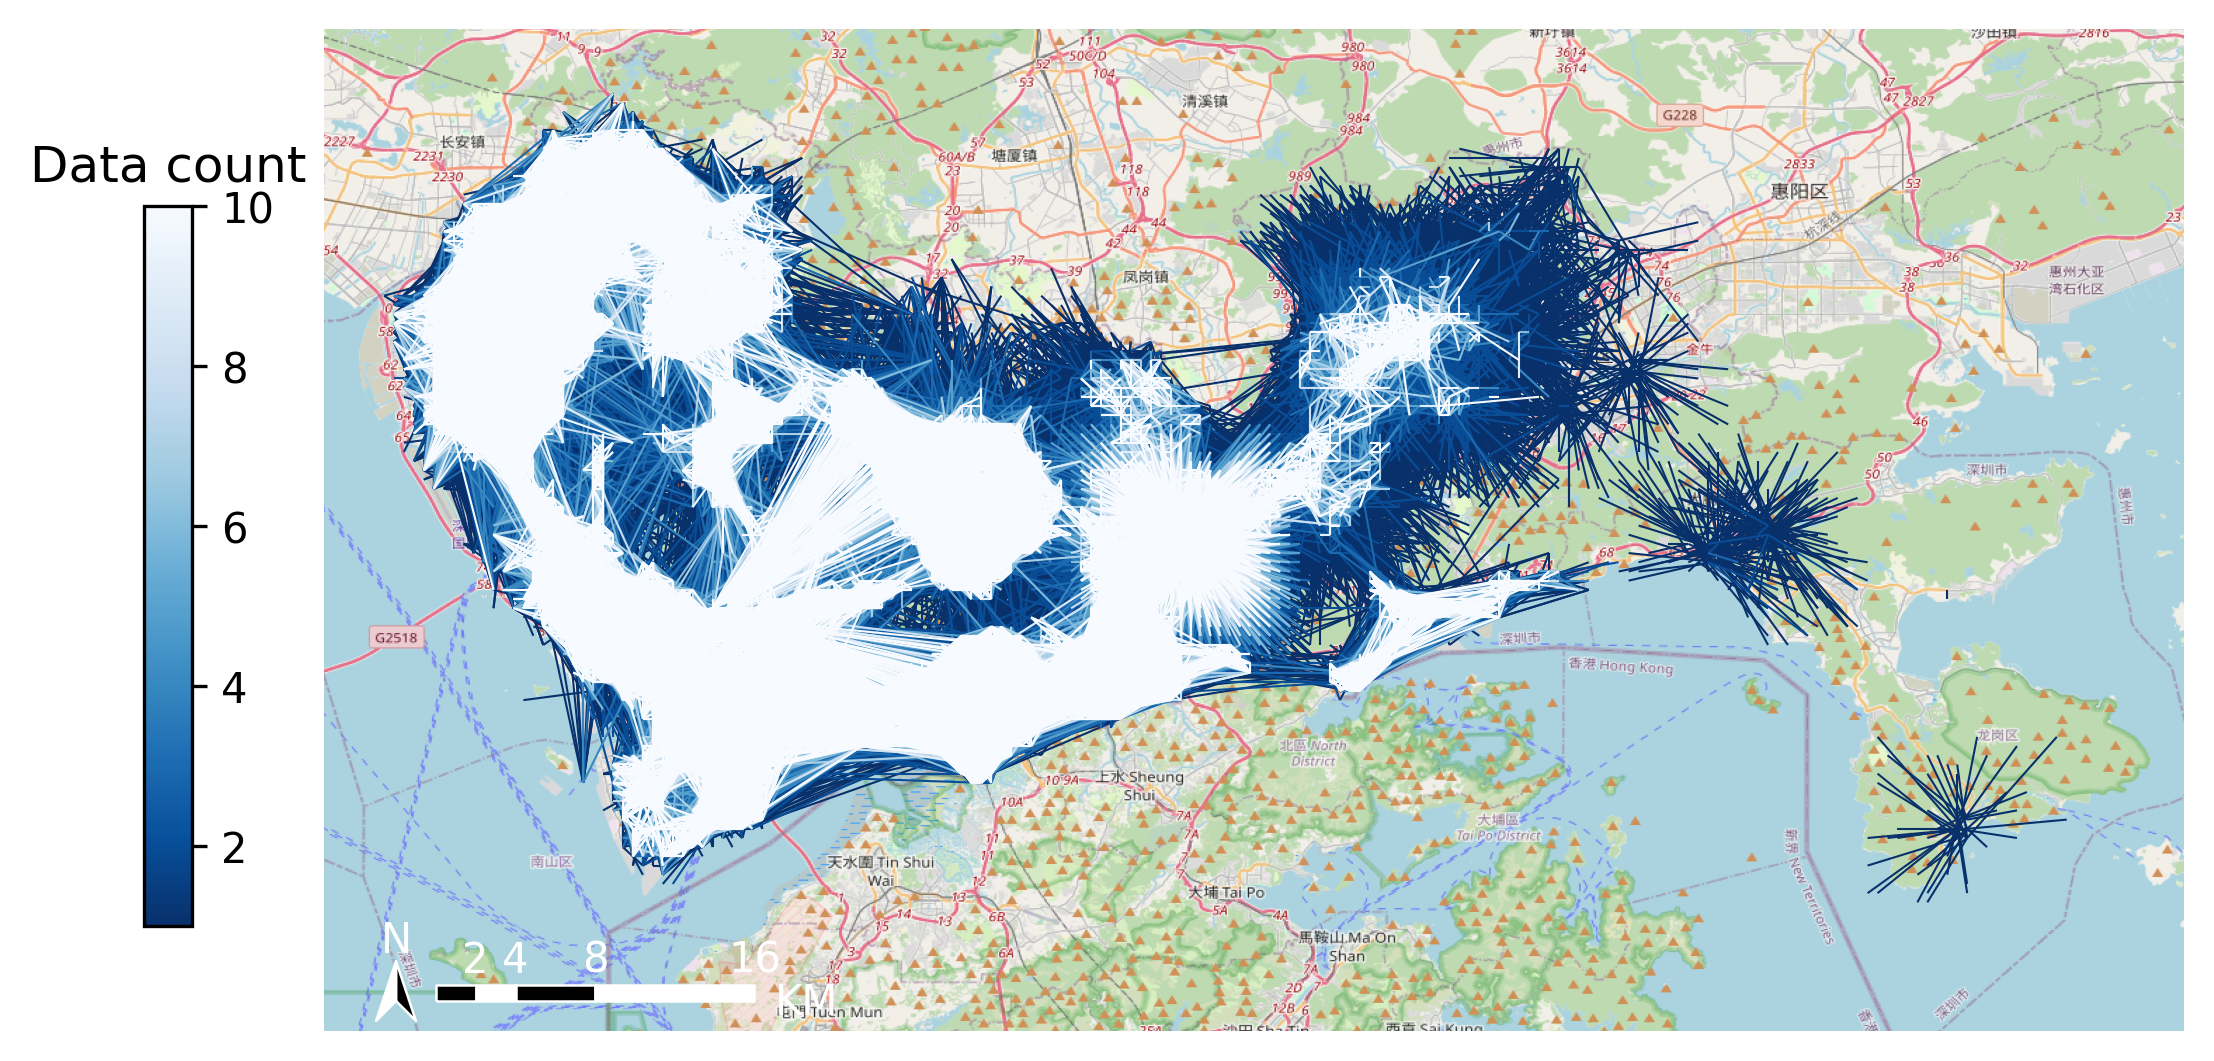
\includegraphics[width= \linewidth]{Figs/栅格流量图.png}
    \caption{深圳市当周共享单车流量分布图}
    \label{fig:流量}
\end{figure}

\subsection{地理因素}

过上述处理后,我们得到的特征主要是关于时间因素,接下来对地理环境因素进行挖掘。

为了更好地表征栅格周边的社会地理环境,我们选取了 9 类常见的 POI(兴趣点)地物进行分析。这些 POI 类型包括公交站点、写字楼、公园、商场、地铁站、居民区、医院、学校和工厂,它们基本涵盖了市民日常活动的主要场所,并且是共享单车流动的重要节点。这些地点的位置及其属性信息对于理解并预测栅格的单车使用模式具有重要影响。

具体来说,POI 数据反映了与人类生活和社会经济活动紧密相连的空间实体,不仅提供了各类职能设施的确切位置,还附带了丰富的关联属性信息。由于其样本量大且信息详尽的特点,POI 数据能够有效而直观地展示城市中不同区域的社会地理特征。


首先利用空间同位规则分析法分析 9 类 POI(兴趣点)地物与电子围栏停车点分布的相关性。通过计算条件概率,得到其同位关系矩阵图(见图\ref{fig:POI})。
\begin{figure}[H]
    \centering
    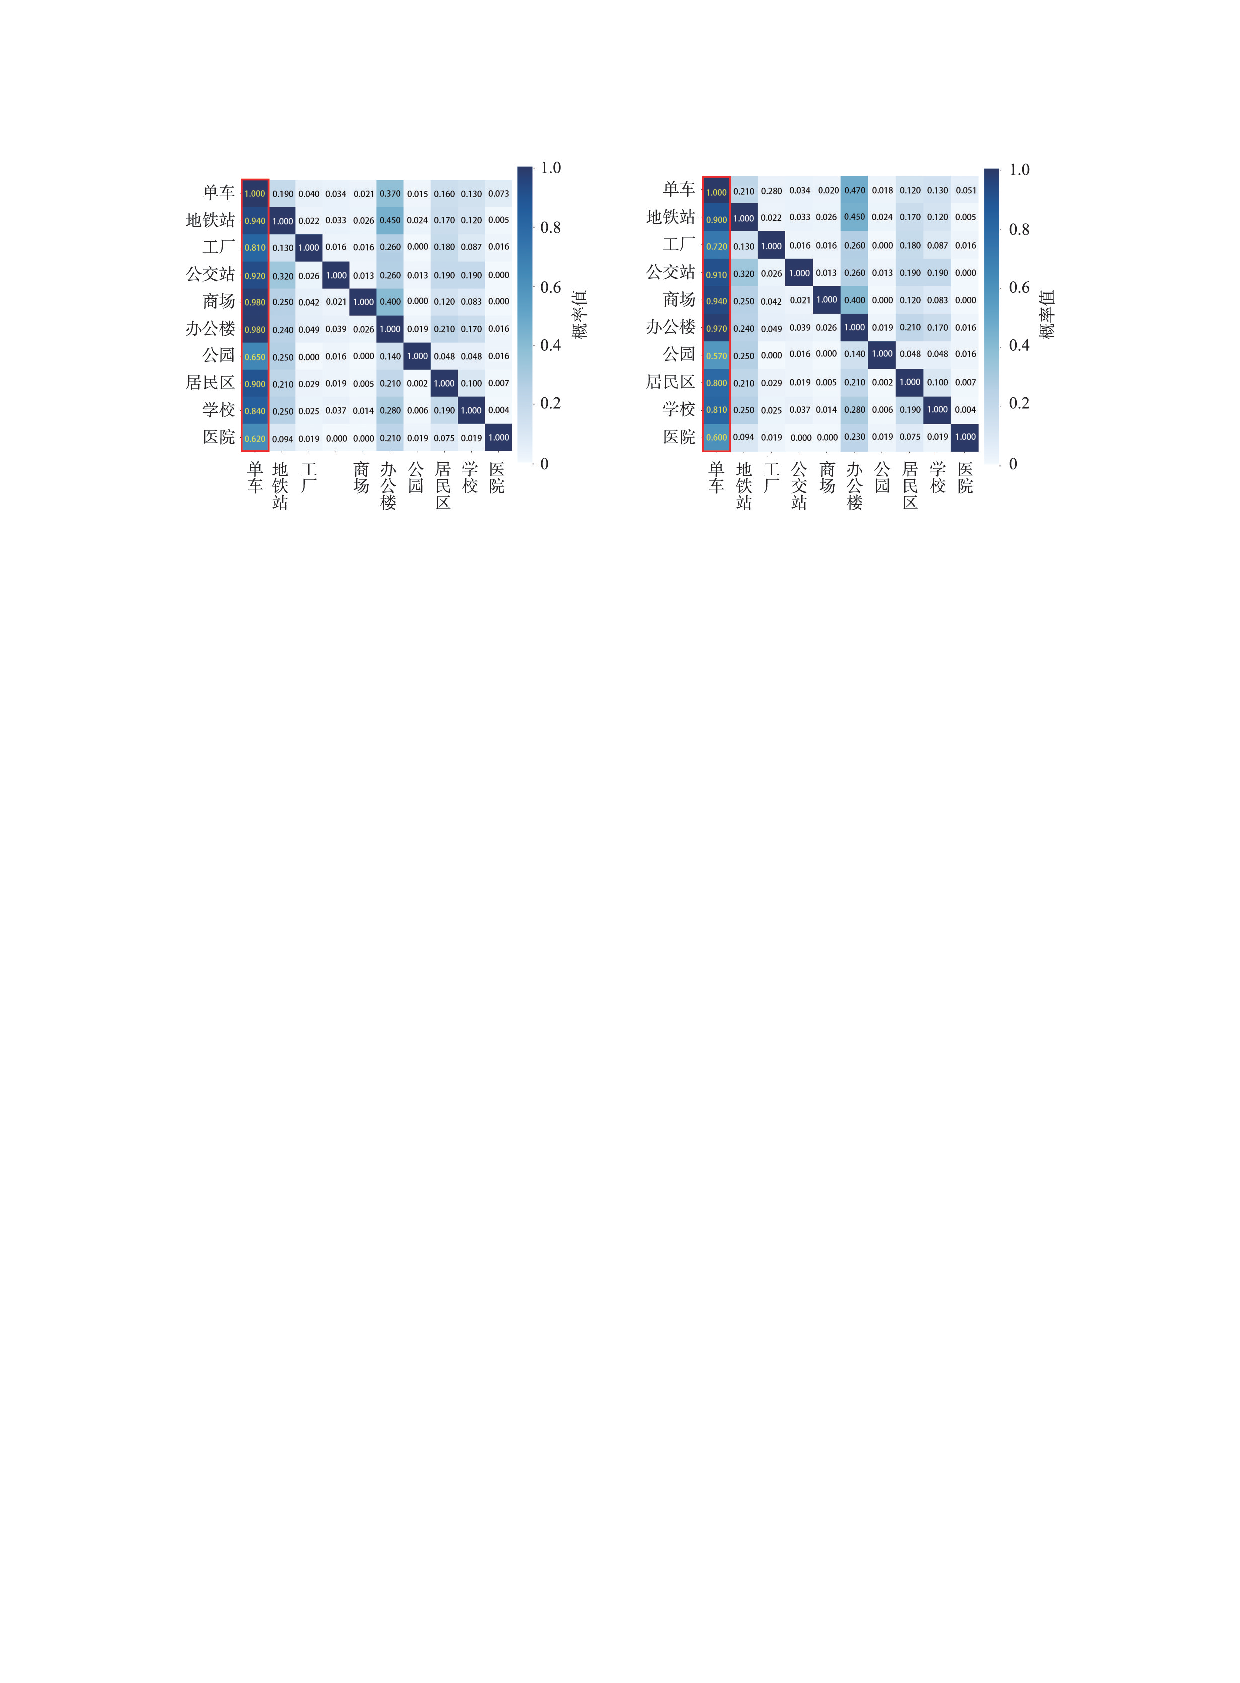
\includegraphics[width=\textwidth]{Figs/各类POI点与共享单车出发停止同位关系矩阵.pdf}
    \caption{各类POI点与共享单车出发(左)停止(右)同位关系矩阵}
    \label{fig:POI}
\end{figure}
图中:第一列表示该 9 类 POI 地物周围100米范围内存在共享单车的概率。从图中可以看出,大部分地点的概率值均在 0.6 以上,特别是商场、办公楼、公交站、地铁站等热点区域的概率值高于 0.9,表明厦门岛地区共享单车的普及率较高,且与这些 POI 地物之间具有较强的空间相关性。

为了进一步量化 POI 数据对各停车点单车使用的影响,本文采用了核密度分析方法来计算每个栅格点周围各类 POI 对栅栏内的影响程度,并将这一影响量化为停车点 POI 指数。具体的计算公式如下:
\begin{equation}
D = \frac{1}{(\text{radius})^2} \sum_{i=1}^{l} \left[ \frac{3}{\pi} \left( 1 - \left( \frac{\text{dist}_i}{\text{radius}} \right)^2 \right)^2 \right] \quad \text{For } \text{dist}_i < \text{radius}    
\end{equation}


式中:$ i = 0, 1, \cdots, l $表示输入的某类POI的所有点;$\text{dist}_i$ 是点 $ i $ 与 $(x, y)$ 之间的距离;$\text{radius}$ 是该类POI的搜索半径,依据下式计算得到。

\begin{align}
\text{radius} &= 0.9 \times \min\left(\text{SD}, \sqrt{\frac{1}{\ln(2)} \times D_m}\right) \times I^{-0.2} \\
D_m &= \frac{\sum_{i=1}^{l} \sqrt{(x_i - x_m)^2 + (y_i - y_m)^2}}{l}\\
\text{SD} &= \sqrt{\frac{\sum_{i=1}^{l} (x_i - x_m)^2}{l} + \frac{\sum_{i=1}^{l} (y_i - y_m)^2}{l}}
\end{align} 

式中:$(x_i, y_i)$ 为点 $i$ 的地理位置坐标;$(x_m, y_m)$ 为该类 POI 的中心点;$D_m$ 计算的是到中心点的平均距离;$\text{SD}$ 计算的是到中心点的标准距离。

利用上述方法,计算深圳市所有栅格受该 9 类 POI 的影响程度,将其称为栅格的 POI 指数,结果如下:
\begin{align}
POI_{\text{index}, i} = [ & D_i^{\text{bus-station}}, D_i^{\text{office}}, D_i^{\text{park}}, \notag\\
& D_i^{\text{mall}}, D_i^{\text{substation}}, 
D_i^{\text{resident}}, \notag\\
& D_i^{\text{hospital}}, D_i^{\text{school}}, D_i^{\text{factory}} ]
\end{align}

式中 $POI_{\text{index}, i}$ 即为停车点 $s_i$ 的 POI 指数,其中 9 个变量分别表示 9 类 POI 类别的指数。

POI 指数实际上反映了各个停车点的社会地理环境特征。对于距离较近的停车点,其 POI 指数通常会较为相似;而即使是距离较远的停车点,只要周边的社会地理环境相似,其 POI 指数也可能接近。因此,使用 POI 指数来衡量电子围栏停车点的相似性,比单纯依赖距离信息能够提供更加丰富和全面的衡量依据。


\section{数据建模分析}

\subsection{已有数据建模方法的局限}

在处理共享单车聚类的问题时,传统方法主要依赖于划分聚类和层次聚类技术。K-means 算法要求预先设定聚类的数量,并且其聚类过程仅基于距离因素;相比之下,DBSCAN 算法通过定义栅格的邻域半径与最小密度阈值来识别单车聚集的热点区域,该算法对点密度非常敏感。不过,由于城市不同功能区及人流分布的影响,自行车栅格的密度并不均匀,这导致了 DBSCAN 聚类结果的精度较低且具有一定的随机性。层次聚类同样在一定程度上取决于密度参数的选择。

这些传统的聚类方法大多侧重于空间特征,较少结合时间维度进行分析,因此所形成的类别较为单一。实际上,影响共享单车使用模式的因素是多方面的,包括但不限于栅格的具体位置、各栅格之间的流动性以及周边地理环境的相似性等空间因素,还有如栅格的历史使用频率这样的时间特征。为了使聚类结果更贴近实际情况,应该综合考虑这些时空要素,以构建更为丰富和准确的特征信息体系(姜晓,2022)\cite{姜晓2022潮汐}。

\subsection{基于时空约束的网络图聚类算法}

在以上研究基础上,本文实现了基于时空约束的网络图聚类算法\cite{姜晓2022潮汐}。该算法计算步骤包括3个部分:栅格相关性网络构建、基于时空约束的网络聚类、社区中心选择。

\subsubsection{栅格相关性网络构建}

栅格之间的关系可以建模成一个相关性网络 $G =(V, E)$ ,其中$V =(s_1,\cdots, s_N)$ 表示 $N$ 个栅格的集合,$E$ 是2个栅格之间连线的集合。具体考虑因素及计算流程如下:
\begin{enumerate}
\item 栅格距离因素

根据地理学第一定律,相近的事物关联更为紧密。因此,考虑距离是限制共享单车区域划分的首要因素。根据停车站点间的空间距离来判断其是否邻接,使用等式\ref{eq:dis}表示邻接情况

\begin{equation}\label{eq:dis}
wD_{i,j} = 
\begin{cases} 
1 & \text{if } \operatorname{dist}(s_i, s_j) \leq R_t \\
0 & \text{if } \operatorname{dist}(s_i, s_j) > R_t 
\end{cases}
\end{equation}

式中:$dist(s_i,s_j)$表示 2 个栅格中心之间的距离;$R_t$为距离阈值。若两站点间距离中 $dist(s_i,s_j)$不大于$dist(s_i,s_j)$,判定其邻接,否则判定其不邻接。通过调节该阈值,控制聚类算法的尺度,从而控制每个聚类区域的大小。在实际计算过程中,我们只需计算 Minkowski 距离即可。

\item 社会地理环境与历史订单因素

使用 POI 指数 $POI\_index_i$ 和历史订单数据 $spacetime_s^t$ 表征栅格内部社区地理环境和时间因素。计算方法如下:

\begin{equation}
\left\{
\begin{aligned}
E_p(s_i, s_j) &= \frac{1 + \rho_p(s_i, s_j)}{2} \\
H_o(s_i, s_j) &= \frac{1 + \rho_o(s_i, s_j)}{2}
\end{aligned}
\right.
\end{equation}

式中:$\rho_p(s_i, s_j)$, $\rho_o(s_i, s_j)$ 分别为两栅格 POI 指数和历史订单数据的 PEARSON 相关性系数,将其正则化到 $[0,1]$ 之间得到 $E_p(s_i, s_j)$ 和 $H_o(s_i, s_j)$。通过 $\mu \in [0,1]$ 控制各自权重大小,得到社会地理环境和历史订单因素的综合权重如下:

\begin{equation}
wEH(s_i, s_j) = \mu E_p(s_i, s_j) + (1 - \mu) H_o(s_i, s_j)
\end{equation}

\item 相关性网络构建

将以上 3 大影响因素进行综合,得到栅格 $(s_i, s_j)$ 间的边权矩阵 $\boldsymbol{W}(s_i, s_j)$,如式(10)所示。

\begin{equation}
\boldsymbol{W}(s_i, s_j) = wD_{i,j} \times wEH(s_i, s_j)
\end{equation}
\end{enumerate}

最终计算所有栅格两两之间的边权 $\boldsymbol{W}(s_i, s_j)$ 得到栅格相关性网络 $G$,此网络中蕴含了栅格之间位置、社会环境和历史订单之间的相似性。得到局部图如下所示:
\begin{figure}[H]
    \centering
    \includegraphics[width=0.8\textwidth]{Figs/边权矩阵局部图.pdf}
    \caption{边权矩阵局部图}
    \label{fig:weightmart}
\end{figure}

\subsubsection{基于时空约束的网络聚类}

在栅格相关性网络构建基础上,进行栅格的聚类划分,将具有相似单车使用特征的栅格聚成同一簇,可以类比成网络图结构中经常使用的社区探测问题。
\begin{figure}[H]
    \centering
    \subfloat[社群假想分布]{
        
\includegraphics[width=0.40\textwidth]{Figs/计算边权矩阵后的社群假想分布.pdf}
        \label{fig:society1}
    }
    \subfloat[算法示意图]{
        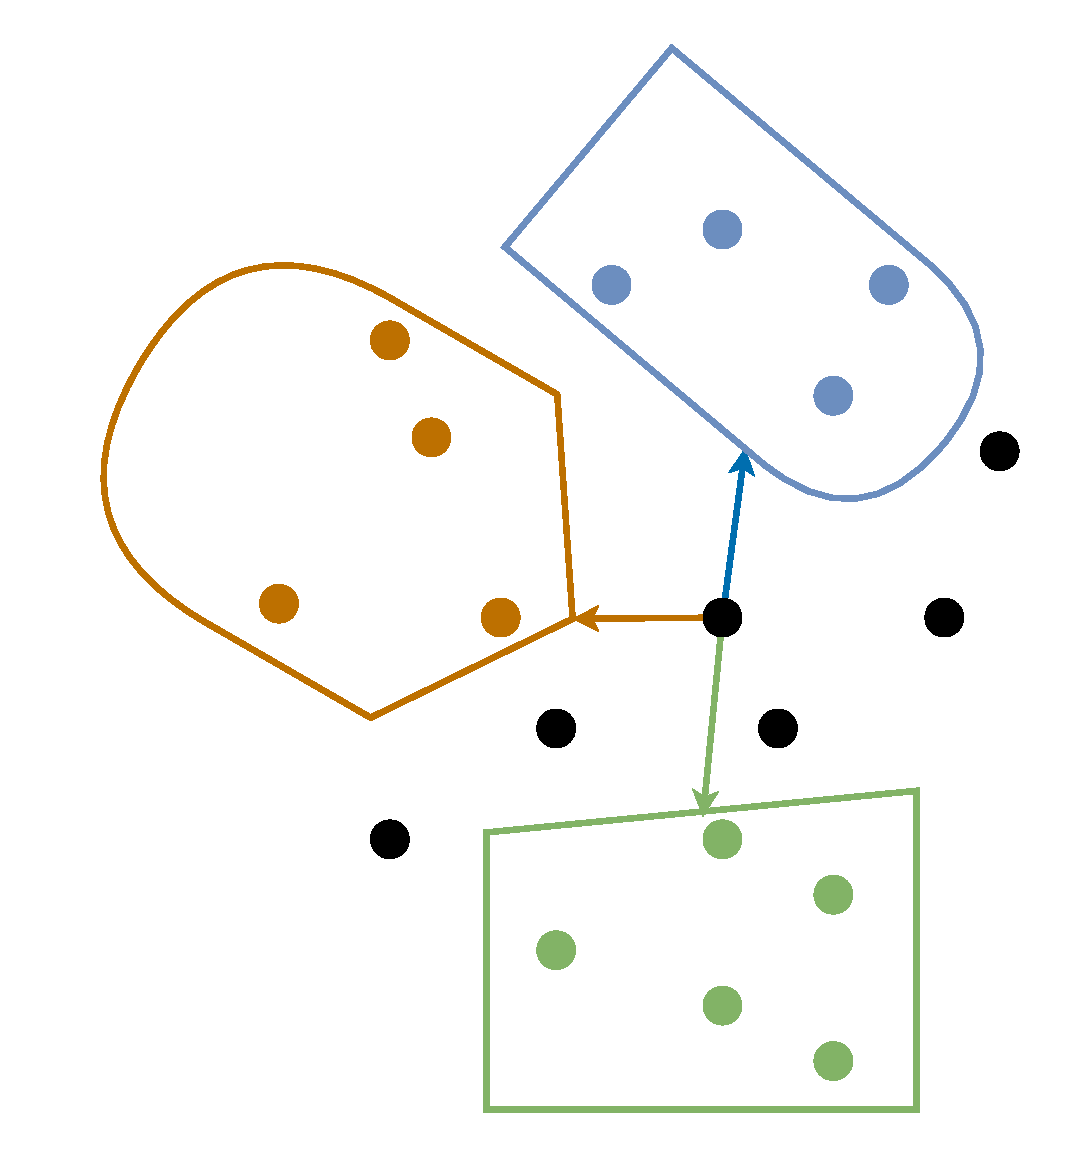
\includegraphics[width=0.48\textwidth]{Figs/算法假想示意.pdf}
        \label{fig:society2}
    }
    \caption{时空因素展示图}
    \label{fig:时空因素展示图}
\end{figure}

\input{Algorithms/算法描述}

过迭代运算,算法贪心地将每个栅格分配到收益 value 最大的邻接簇中,直到所有栅格不在簇间移动,从而完成栅格的聚类。

算法流程如下:
\input{Algorithms/基于时空约束的网格聚类}

\subsubsection{社区中心选择}

基于时空约束的网络图聚类划分本质上是一种图的社区划分,并没有进行聚类中心的计算。本研究社区中心的选择主要考虑2个因素:度中心性和接近中心性。

度中心性用于反映节点在整个网络中的重要程度,为节点 $v_i$ 的度与网络节点个数比值,即:

\begin{equation}
DC(i) = \frac{\sum\limits_{j=0}^{N} w_{ij}}{N-1}
\end{equation}

式中:$w_{ij}$ 为相关性矩阵中的边权;$N$ 为网络中所有节点的个数。在网络中,栅格的度越大,说明该栅格与其他栅格关联程度越高。

接近中心性用于表达栅格在其所属社区中的中心化程度,计算如式(16)所示。

\begin{equation}
CC(i) = \frac{n_c - 1}{\sum\limits_{j} d_{ij}}
\end{equation}

式中:$n_c$ 为当前社区中节点的个数;$d_{ij}$ 为节点之间的距离。在社区中,接近中心性越大说明该点与其他点越接近,中心化程度越高。

最后,将上述2个指标归一化到 $[0,1]$ 后相加,取社区中计算结果最大的节点作为该社区的中心,该中心综合了社区内部的接近性及其与临近社区的关联性,相较其他节点更具代表性,可作为共享单车区域的中心代表。

\section{实验与结果分析}

\subsection{全市尺度聚类结果分析}

在全市尺度上,使用基于时空尺度的图聚类算法,将距离阈值设置 500 m,进行聚类,结果如图 \ref{fig:wholecity} 所示,全岛停车点被划分成了 19 个社区。

\begin{figure}[H]
    \centering
    \includegraphics[width=\textwidth]{Figs/全市尺度聚类结果分析.pdf}
    \caption{全市尺度聚类结果与分析}
    \label{fig:wholecity}
\end{figure}


可以发现,如图中蓝色蓝色部分,社区中心呈现一定聚集性特征,说明该算法对于社区中心的选择既考虑了社区内部的联系,也综合了周边社区的影响。

图中红色圈所圈黄色类的范围为了驻扎大量科技工业园区,该公园周边的栅格被高速公路在距离上分隔开,但由于科技园周边具有相似的社会地理环境特征,并且周边单车在使用时间上也具有相似性,所以被划分到了同一社区内,说明相较传统算法,该方法不仅考虑了距离因素,同时也综合了地理环境和历史订单因素。

同理,红色圈所圈蓝色类为盐田国际集装箱码头,紫色区为沙头角保税区,二者共享单车的面向对象并不重叠,故被分成两簇,再次验证了该方法的科学性。

事实上,我们也运用了 K-means 算法进行聚类,共分为 21 个社区,结果如下
\begin{figure}[H]
    \centering
    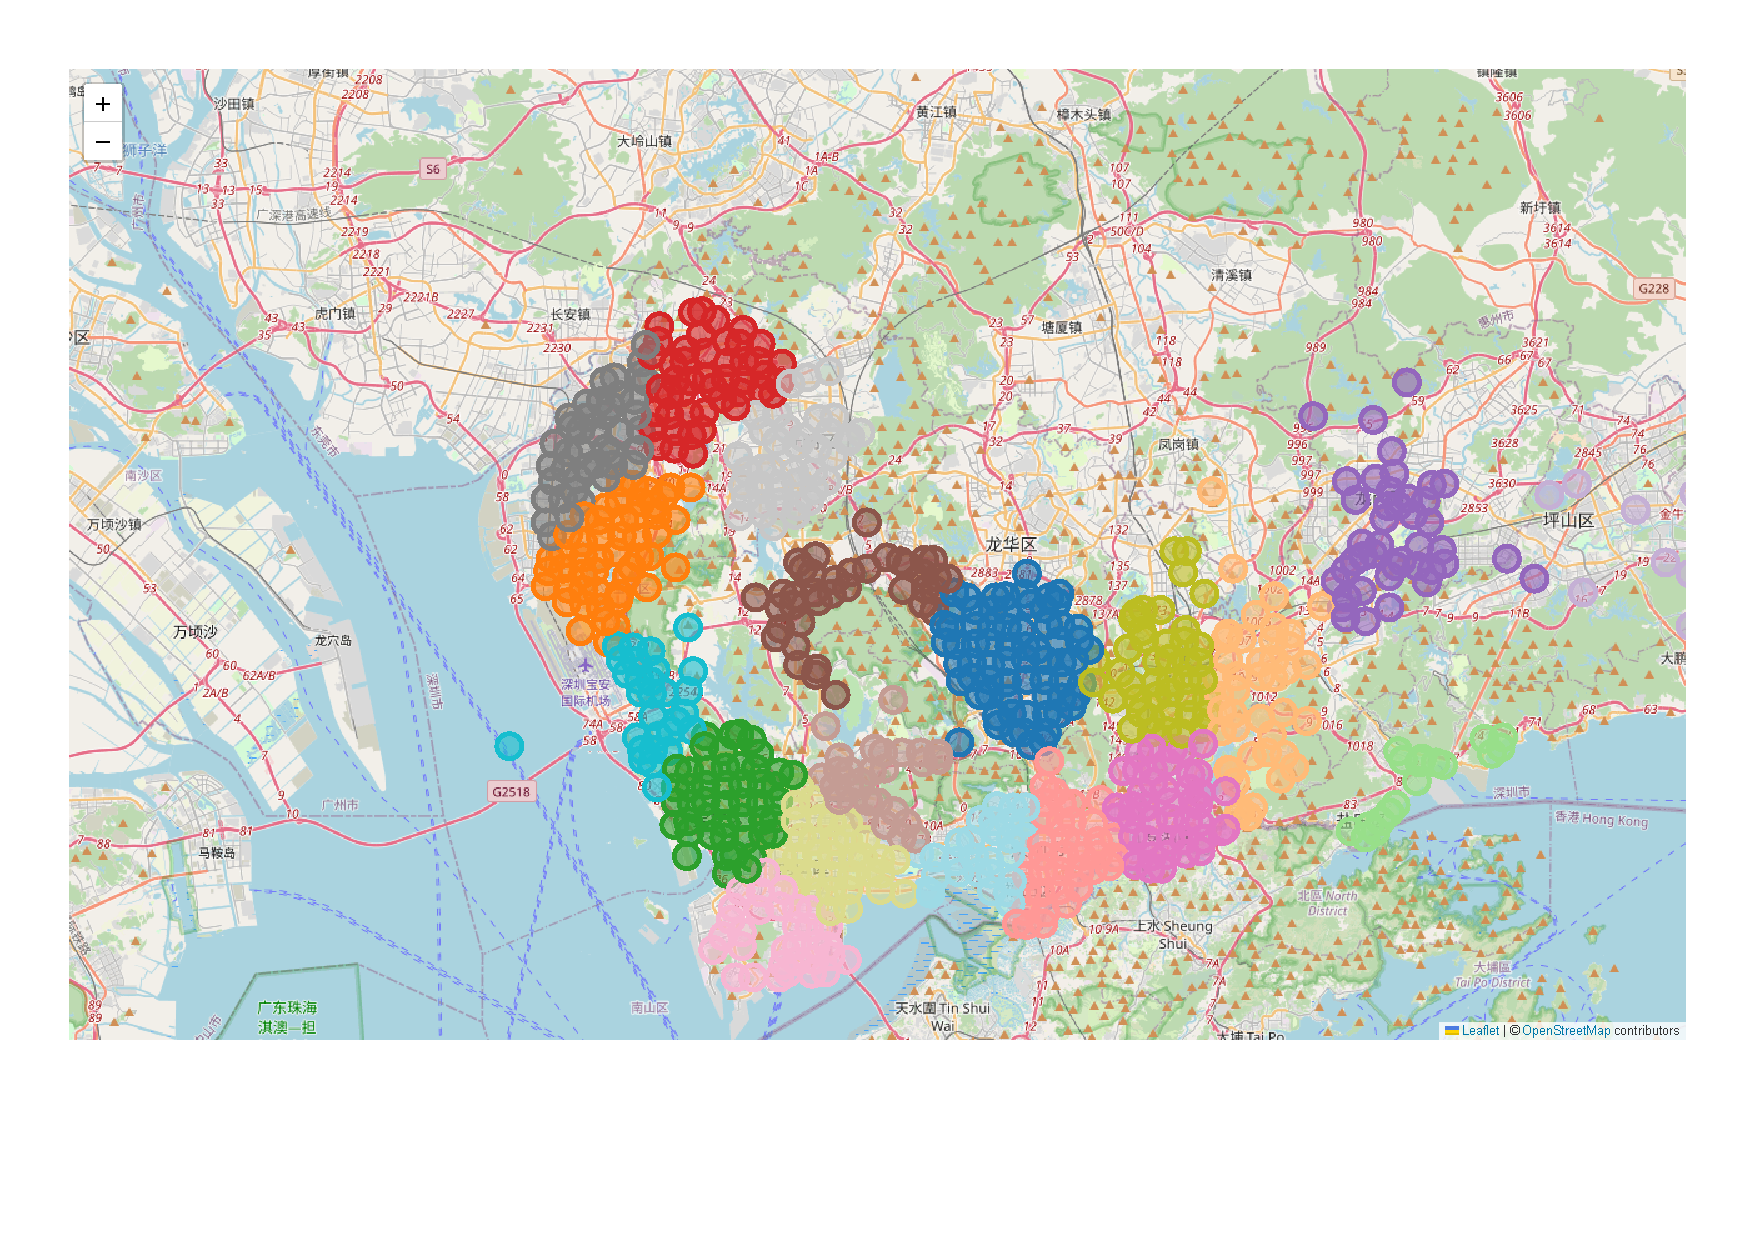
\includegraphics[width=\textwidth]{Figs/kmeans.pdf}
    \caption{基于Kmeans聚类的结果}
    \label{fig:kmeans}
\end{figure}

可见, Kmeans 算法聚类效果并不并不理想,对于距离和历史订单因素的考虑有所欠缺。更重要的是,K-means的运行时间将近 3h,而基于时空约束的网格聚类时间不超过 30 min,足以见得算法的优越性。
\subsection{栅格尺度流量结果分析}
单车流动情况是单车调度工作需要考虑的重要因素,本研究统计了全部19个区域单车订单的历史数据,并将 8月 13号当天各个栅格的流量(流出)数据绘制如下:
\begin{figure}[H]
    \centering
    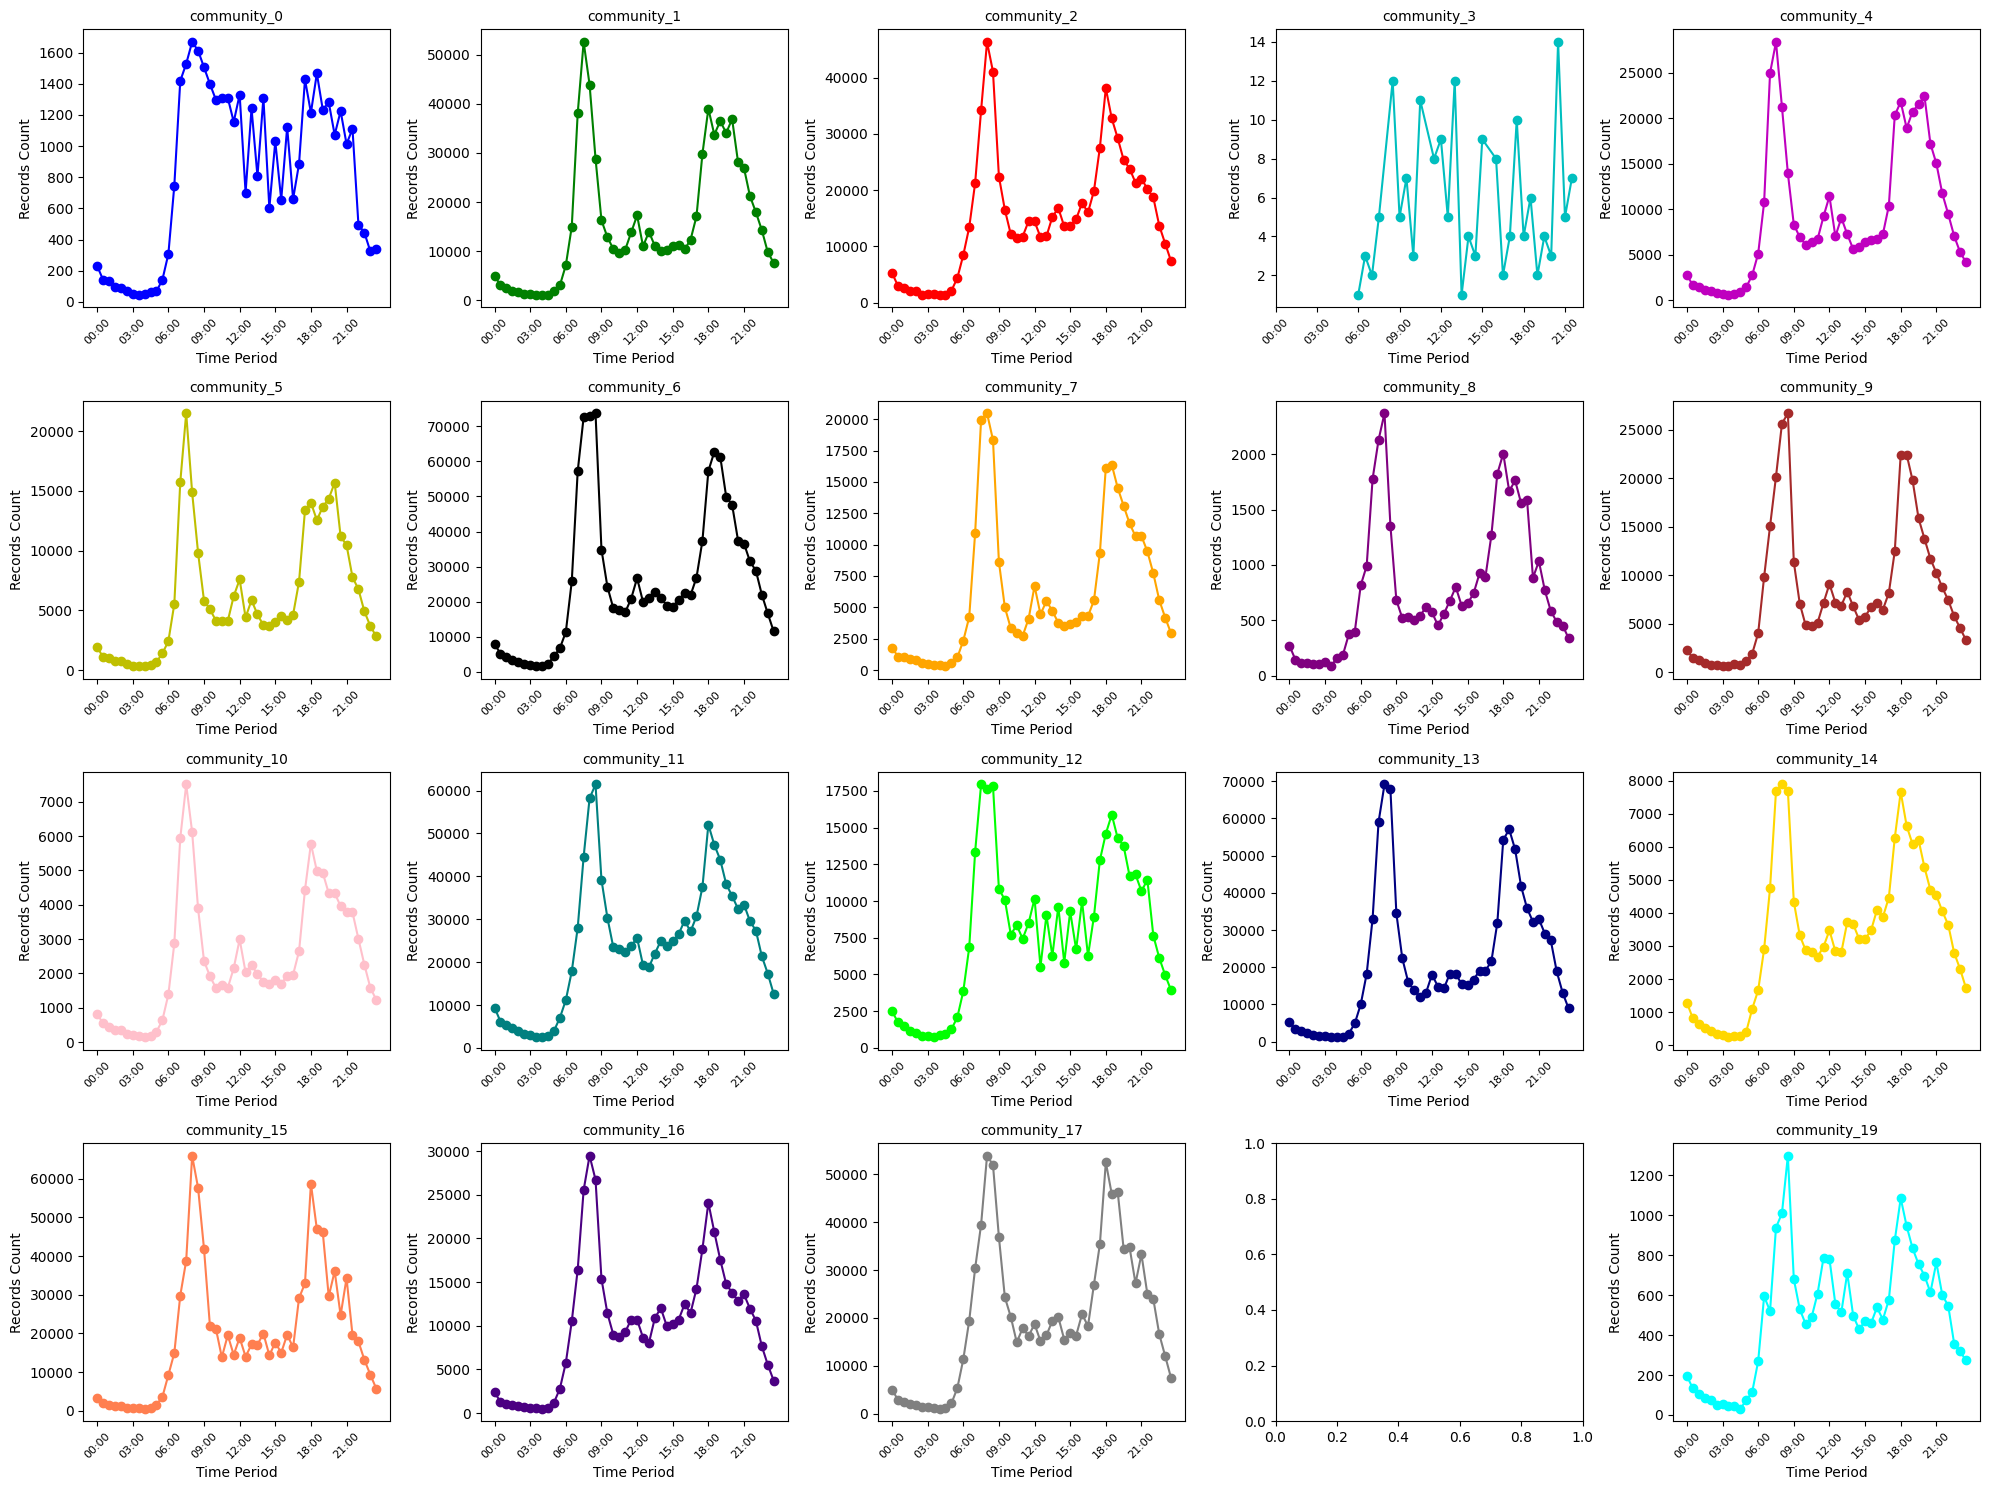
\includegraphics[width=1\textwidth]{Figs/局部流量变化分析.png}
    \caption{19个栅格8月13日流量变化}
    \label{fig:grid}
\end{figure}

我们发现:
\begin{enumerate}
\item 由于识别问题,第 19 社区由于 \texttt{Python} 设置问题,往后平移了 1 个单位,但不影响结果分析。

\item 早晚高峰的“潮汐”现象是普遍存在的。在大部分栅格中均出现了“双峰”的图形特征。区别在于规模的大小。

\item 大部分社区的流量高峰对应于上下班时间(例如早晨7-9点,晚上5-7点),反映了通勤行为的共性。而中午时间流量相对较低,可能是因为大部分人处于休息或在固定地点活动。

\item 部分社区凸显出不同于双峰的时间序列,体现在中午时间流量较高,对比地图发现该区域集中分布着商业设施,导致中午对共享单车的需求量较高。


\subsection{区域尺度流量分析}

将各个地区路程、时间、速度分社区绘制分布图,
\begin{figure}[H]
    \centering
    \subfloat[社区聚类的运行距离分布]{
    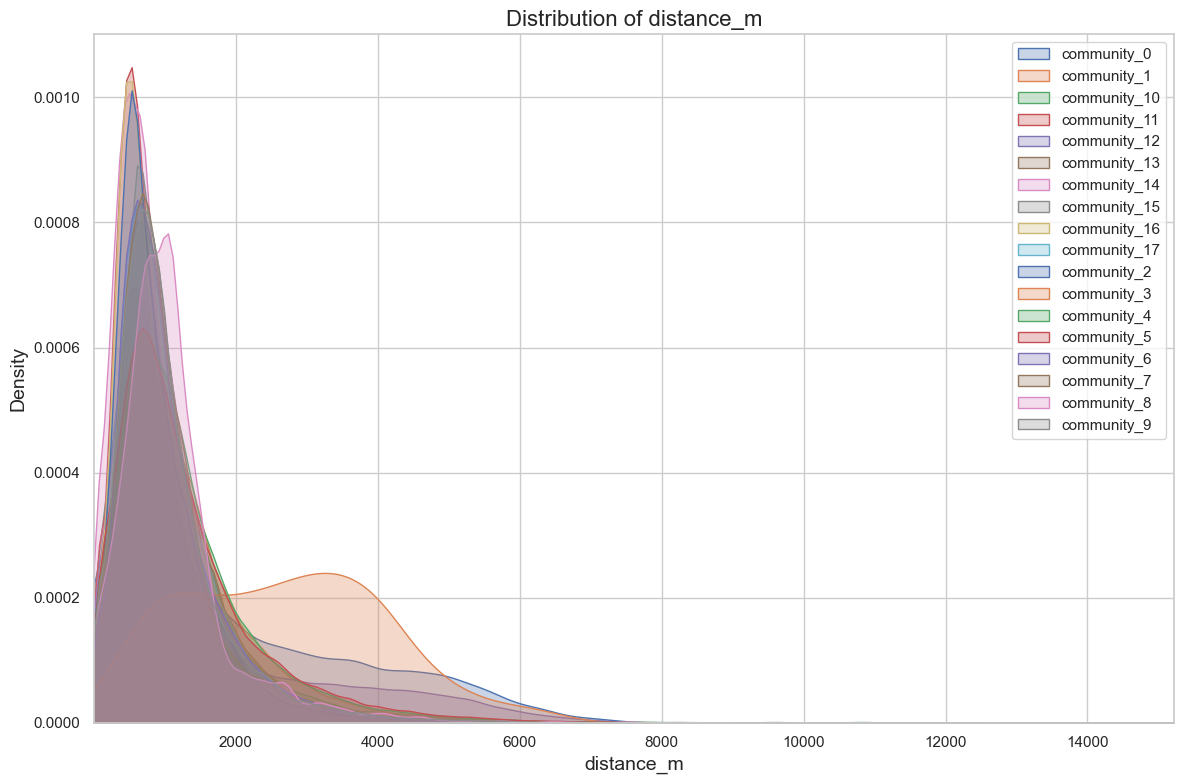
\includegraphics[width = 0.5\textwidth]{Figs/聚类社区的运行聚类分布.png}
    \label{fig:community_dis}
    }
    \subfloat[社区聚类的运行时间分布]{
    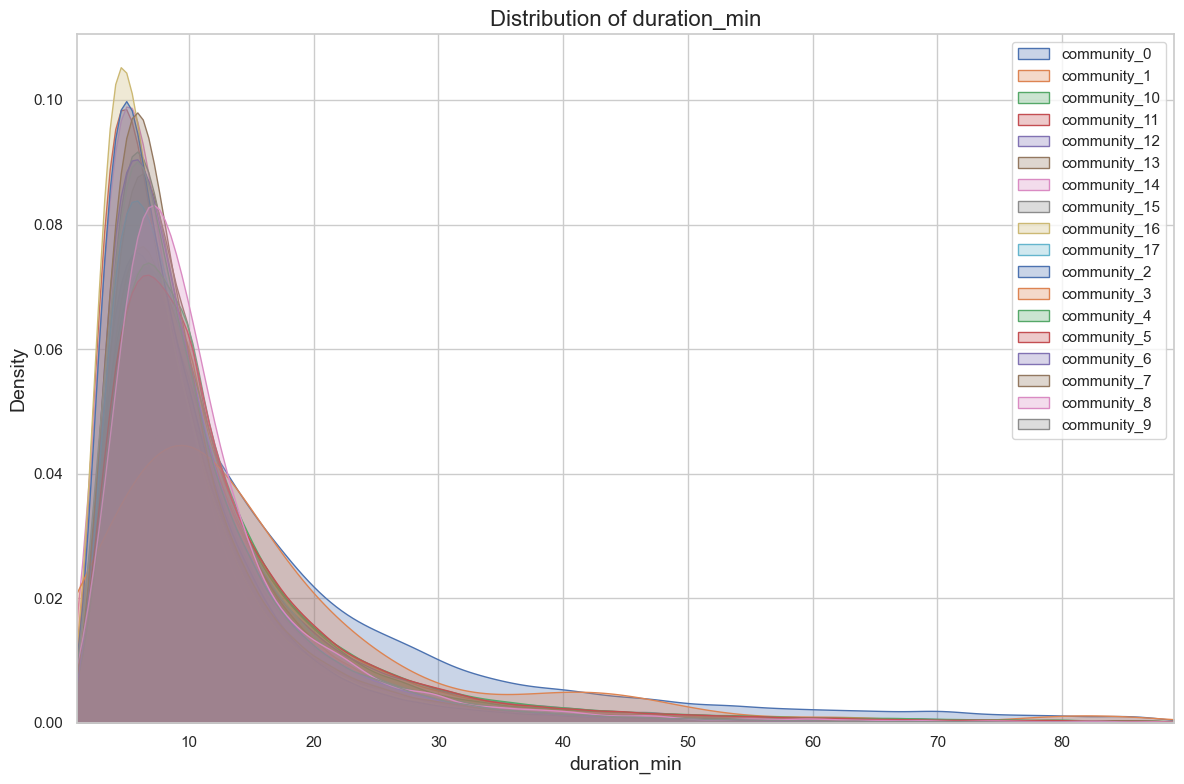
\includegraphics[width = 0.5\textwidth]{Figs/聚类社区的运行时间分布.png}
    }
    \hfill
    \subfloat[聚类社区的运行速度分布]{
        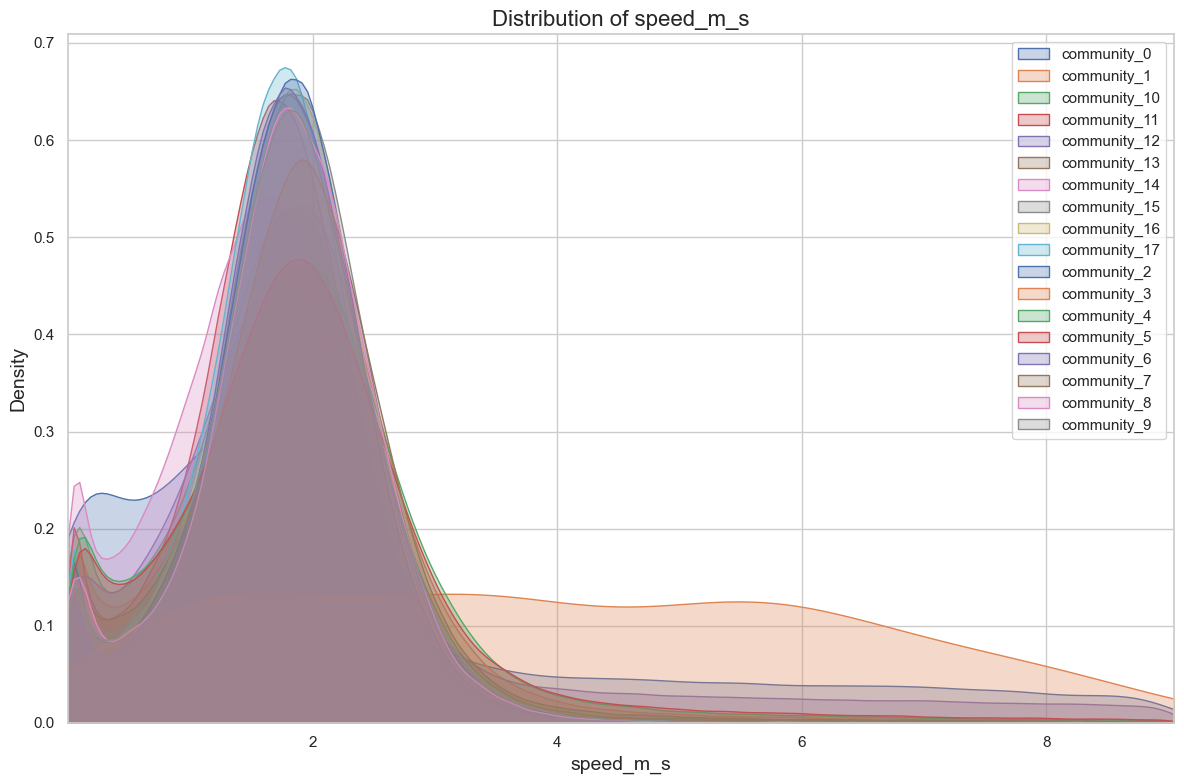
\includegraphics[width= 0.5\textwidth]{Figs/聚类社区的运行速度分布.png}
        \label{fig:community_speed}
    }
\end{figure}
\end{enumerate}


社区1的运行距离和运行速度表现出不同于其他社区的一般分布,这一现象引发了我们对宝安区独特城市化进程的深入思考。经查询,宝安区在改革开放初期是深圳市的一个以农业为主的郊区,随着深圳特区的发展,逐渐转型为工业和制造业的重要基地。近年来,宝安区经历了快速的城市化过程和发展转型,这不仅改变了区域内的产业结构,也深刻影响了居民的生活方式和交通需求。

从数据分析来看,社区 1 展现出的高速度、远距离以及大规模的单车使用特征,暗示着该地区存在显著的人口流动和长距离通勤需求。这种模式可能与宝安区内大量的工业园区、写字楼和住宅区之间的人员往来密切相关。此外,由于宝安区正在经历快速的城市化和基础设施建设,新建的道路网络和公共交通系统的完善也为长距离骑行提供了更好的条件。

基于这些观察,我们可以合理推断,在未来的城市发展中,宝安区将吸引大量的投资和关注。政府可能会继续推动该地区的产业升级和经济多元化,促进高新技术产业和服务业的发展。同时,随着更多企业和机构入驻宝安区,这里的工作机会也将增加,进一步刺激人口流入和居住需求的增长。

对于共享单车运营方而言,针对宝安区的特点调整投放策略显得尤为重要。考虑到社区 1 的特殊性,可以考虑:
\begin{enumerate}
    \item \textbf{增加单车投放量}:为了满足高峰时段的高需求,尤其是在工作日早晚上下班时间,适当增加单车数量,确保用户能够方便快捷地找到可用车辆。
    \item \textbf{推广长距离骑行服务}:鉴于社区1用户偏好较长距离骑行,可以推出专门的长距离骑行套餐或优惠活动,鼓励市民选择更环保的出行方式。
\end{enumerate}

\section{实践价值与展望}

\subsection{实践价值}

在数据预处理方面,通过整合POI数据和订单数据,将不易处理的时间序列数据转化为直观易处理的面板数据,实现了地理栅格化;在实现栅格化的基础上,进一步实现了相关性网络的构建,将栅格之间的位置、社会环境以及历史订单相似信息归一到边权矩阵中,具有可迁移性;之后,类比网络图结构中的社区探测问题,实现了高效的网格聚类,有效探索出不同区域的单车使用情况与流动规律,并发现单车使用热点区域,针对热点区域进行单车潮汐特征挖掘,侧面反映了城市发展潜力,为共享单车短期运营和长期决策提供科学支持。

总之,通过对栅格进行基于时空约束的网格聚类分析,这项研究不仅提升了对城市内单车使用行为的理解,也为提升共享单车服务效率、促进可持续城市发展提供了宝贵的数据支持和理论依据。

\subsection{展望}
\begin{enumerate}
    \item 我们在初步处理大规模数据集便面临了性能瓶颈。未来可以引入更高效的图计算框架(如图神经网络)以及并行计算方法,进一步提升算法的计算效率。

    \item 在运行代码中,有大量的重复性繁琐操作,我们也参考了部分 \texttt{TransBigData,GeoPandas} 的库的操作,可以考虑将操作写成模块的形式,探讨方法的泛化能力和跨城市迁移能力,以提升其在不同场景下的适用性。
    
    \item 本文主要基于时空数据和土地使用类型,未来可以进一步引入更多维度的影响因素,如天气变化、道路条件、居民收入水平等,构建更全面的共享单车使用模型。

    \item  如引言所说,共享单车是城市交通体系的重要组成部分,未来可以进一步研究其与公交、地铁等其他交通方式的协同效应,探索如何通过多模式交通的联动优化,实现城市交通资源的全局最优配置。
\end{enumerate}



\newpage
\bibliography{参考文献}
\newpage

\appendix

\end{document}
